\section{Configurarea aplicatiei}

% -------------------------------------------------- Hardware
\subsection{Configurarea predictorului}
\label{sec:config_hw}

Implementarea OGEHL expune trei parametri configurabili care controleaza
dimensiunea si precizia predictorului. Acestia pot fi modificati din interfata
grafica a aplicatiei inainte de pornirea unei simulari.

\begin{itemize}
    \item \textbf{Numarul de tabele} ($N$) --- Determina cate tabele de
          predictie sunt folosite simultan. Un numar mai mare de tabele
          permite capturarea unor corelatii mai complexe intre branch-uri,
          dar creste consumul de memorie. Valorile acceptate sunt intre
          \textbf{4} si \textbf{12} tabele, valoarea implicita fiind
          \textbf{7}.

    \item \textbf{Marimea tabelelor} --- Reprezinta numarul de intrari per
          tabel. O valoare mai mare reduce probabilitatea de aliasing
          (doua branch-uri diferite care indexeaza acelasi contor), dar
          creste memoria necesara. Valoarea implicita este
          \textbf{2048 intrari}, iar maximul suportat este
          \textbf{88\,000 intrari} (dimensionat astfel incat 12 tabele
          maxime sa nu depaseasca $\approx$1~MB total).

    \item \textbf{Lungimea contoarelor} ($k$) --- Numarul de biti al
          fiecarui contor saturat din tabele. Controarele mai lungi
          reactioneaza mai lent la schimbari de comportament, dar sunt
          mai stabile pe branch-uri cu comportament consistent. Valorile
          acceptate sunt \textbf{3}, \textbf{4} sau \textbf{5} biti,
          valoarea implicita fiind \textbf{4 biti}.
\end{itemize}

Ceilalti parametri interni ai predictorului ($\alpha = 2$, $L_1 = 2$,
$\theta$ initial $= N$) sunt fixati la compilare in
\texttt{bp\_defines.h} si nu sunt expusi in interfata grafica, deoarece
valorile lor sunt optime pentru majoritatea aplicatiilor conform
literaturii de specialitate\cite{seznec2004gehl}. Dupa ordine parametrii sunt:

\begin{itemize}
	\item $\alpha$: factor folosit in calcularea seriei geometrice a lungii istoricului
	\item $L_i$: Lungimea istoricului folosită pentru a adresa tabela $i$. Aceasta e definită ca o serie geometrică având forma:
	\[
	L(i) = \alpha^{i-1} \cdot L(1)
	\]
	\item $\theta$: Prag folosit in comparare cu suma algebrica a contoarelor
\end{itemize}

% -------------------------------------------------- Software
\subsection{Toolchain software}
\label{sec:toolchain}

Proiectul este structurat in doua componente independente, fiecare cu
propriul build target CMake: aplicatia principala si suita de teste de unitate.

\subsubsection*{Aplicatia principala}

Aplicatia este scrisa in C si foloseste doua biblioteci externe pentru
interfata grafica:

\begin{itemize}
    \item \textbf{raylib} --- librarie grafica multiplatforma scrisa in C,
          care ofera suport pentru ferestre, randare 2D/3D si gestionarea
          input-ului. In proiect este folosita ca dependenta de baza,
          link-editat static din \texttt{libs/raylib/lib/libraylib.a}. Link descarcare:  \url{https://https://github.com/raysan5/raylib}
    \item \textbf{raygui} --- biblioteca \cite{raygui} pentru UI in mod imediat (\textit{immediate
          mode GUI}) construita peste raylib, folosita pentru a crea
          toate controalele interfetei (campuri de text, butoane, liste).
          Este inclusa ca fisier header-only direct in sursa. Link descarcare: \url{https://github.com/raysan5/raygui}
\end{itemize}

Alegerea acestor biblioteci a fost motivata de faptul ca libraria
predictorului OGEHL este scrisa in C, astfel incat integrarea unui
toolkit grafic tot in C era solutia cea mai simpla si fara dependente
suplimentare de runtime. Build-ul aplicatiei este gestionat cu
\textbf{CMake}, iar sursa este organizata in directoarele
\texttt{src/bp/} (logica predictorului), \texttt{src/ui/} (interfata
grafica) si \texttt{src/common/} (comunicare inter-thread si
orchestrare).

Exemple de interfata se pot vedea in capitolul \textbf{Ghid de
utilizare}.

\begin{figure}[H]
	\centering
	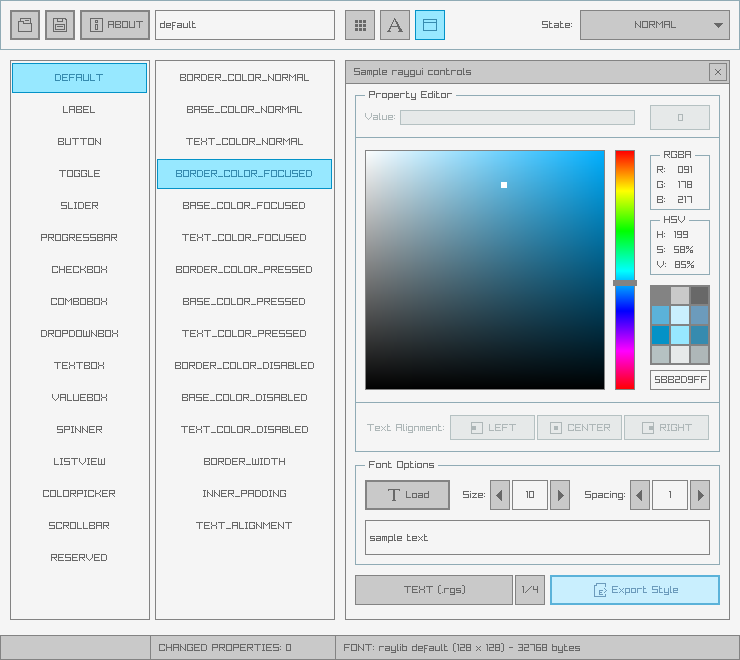
\includegraphics[width=0.75\linewidth]{images/raygui.png}
	\caption{Exemplu UI raygui}
	\label{fig:raygui}
\end{figure}

\subsubsection*{Integrarea cu SimpleScalar}

Pentru integrarea predictorului in SimpleScalar nu au fost necesare
biblioteci externe. Fisierele sursa ale modulului \texttt{bp/} au fost
copiate direct in arborele simplesim si incluse in compilare.

In plus, build-system-ul original al SimpleScalar (bazat pe
\texttt{Makefile}-uri generate manual) a fost inlocuit cu
\textbf{CMake}, iar fisierele sursa au fost reorganizate in structura
conventionala \texttt{src/} / \texttt{inc/}, facilitand navigarea
codului si integrarea cu unelte moderne de analiza statica si
debugging.
